s\chapter{DEVELOPMENT OF THE iOS APP}
\label{chap:development of the app}

The development of the iOS app is divided into two areas which are :

\begin{itemize}
    \item Front-end
        \begin{itemize}
            \item App designing
            \item Mobile App screens and their significance
        \end{itemize}

    \item Back-end
        \begin{itemize}
            \item Process of getting data from NASA's server
            \item Web services required for \gls{json} parsing between database and the front-end
        \end{itemize}
    
     \item API Usage
        \begin{itemize}
            \item Major APIs used
        \end{itemize}    
\end{itemize}

\section{FRONT-END OF THE APP}

\subsection{App Designing}
    
\centerline{\textbf{Xcode - IDE}}

\centerline{Xcode 9.3 has been used for the development of the app}

\textbf{Xcode} is an Integrated Development Environment, which implies it pulls every one of the instruments expected to create an application (especially a content tool, a compiler, and a manufacture framework) into one programming bundle instead of abandoning them as an arrangement of individual devices associated by contents. Xcode is Apple's authentic \gls{ide} for \gls{mac} and \gls{iOS} engineers. It was initially known as Project Builder in the NeXT days, and renamed to Xcode some place around Mac OS X 10.3 or 10.4. By adaptation 4, Apple had collapsed in the sidekick Interface Builder program so there was just a single application package; the plan of the program hasn't changed a ton from that point forward, albeit clearly the instruments are refreshed routinely. \\

%add to this biblipography as my copying from apple's website.

Apple provides Built-In Interface Builder in the \gls{ide} for designing.
According to Apple's website, The Interface Builder editor within Xcode makes it simple to design a full user interface without writing any code. Simply drag and drop windows, buttons, text fields, and other objects onto the design canvas to create a functioning user interface. \\

Because Cocoa and Cocoa Touch are built using the Model-View-Controller pattern, it is easy to independently design your interfaces, separate from their implementations. User interfaces are actually archived Cocoa or Cocoa Touch objects (saved as .nib files), and \gls{macOS} and \gls{iOS} will dynamically create the connection between \gls{ui} and code when the app is run. \\

%add to this biblipography as my copying from apple's website.
%https://developer.apple.com/library/archive/documentation/General/Conceptual/Devpedia-CocoaApp/Storyboard.html
As you know, i have used built in feature of Xcode for designing. Apple also provides one more tool for visualization of the design which is \textbf{Storyboard}. \\ \\
According to Apple, A storyboard is a visual representation of the user interface of an \gls{iOS} application, showing screens of content and the connections between those screens. A storyboard is composed of a sequence of scenes, each of which represents a view controller and its views; scenes are connected by segue objects, which represent a transition between two view controllers. \\

Xcode provides a visual editor for storyboards, where you can lay out and design the user interface of your application by adding views such as buttons, table views, and text views onto scenes. In addition, a storyboard enables you to connect a view to its controller object, and to manage the transfer of data between view controllers. Using storyboards is the recommended way to design the user interface of your application because they enable you to visualize the appearance and flow of your user interface on one canvas. Figure 4.1 shows the storyboard of the app. 

Some of the advantages of using Storyboard are mentioned below:-
\begin{itemize}
    \item It's a container for all your Scenes (View Controllers, TabBar Controllers and more).
    \item A director of associations and transitions between these scenes (called Segues).
    \item It gives you the chance to see what My view will look like at runtime without running your application.
\end{itemize}

\newpage

    \begin{figure}[H]
            \centering
            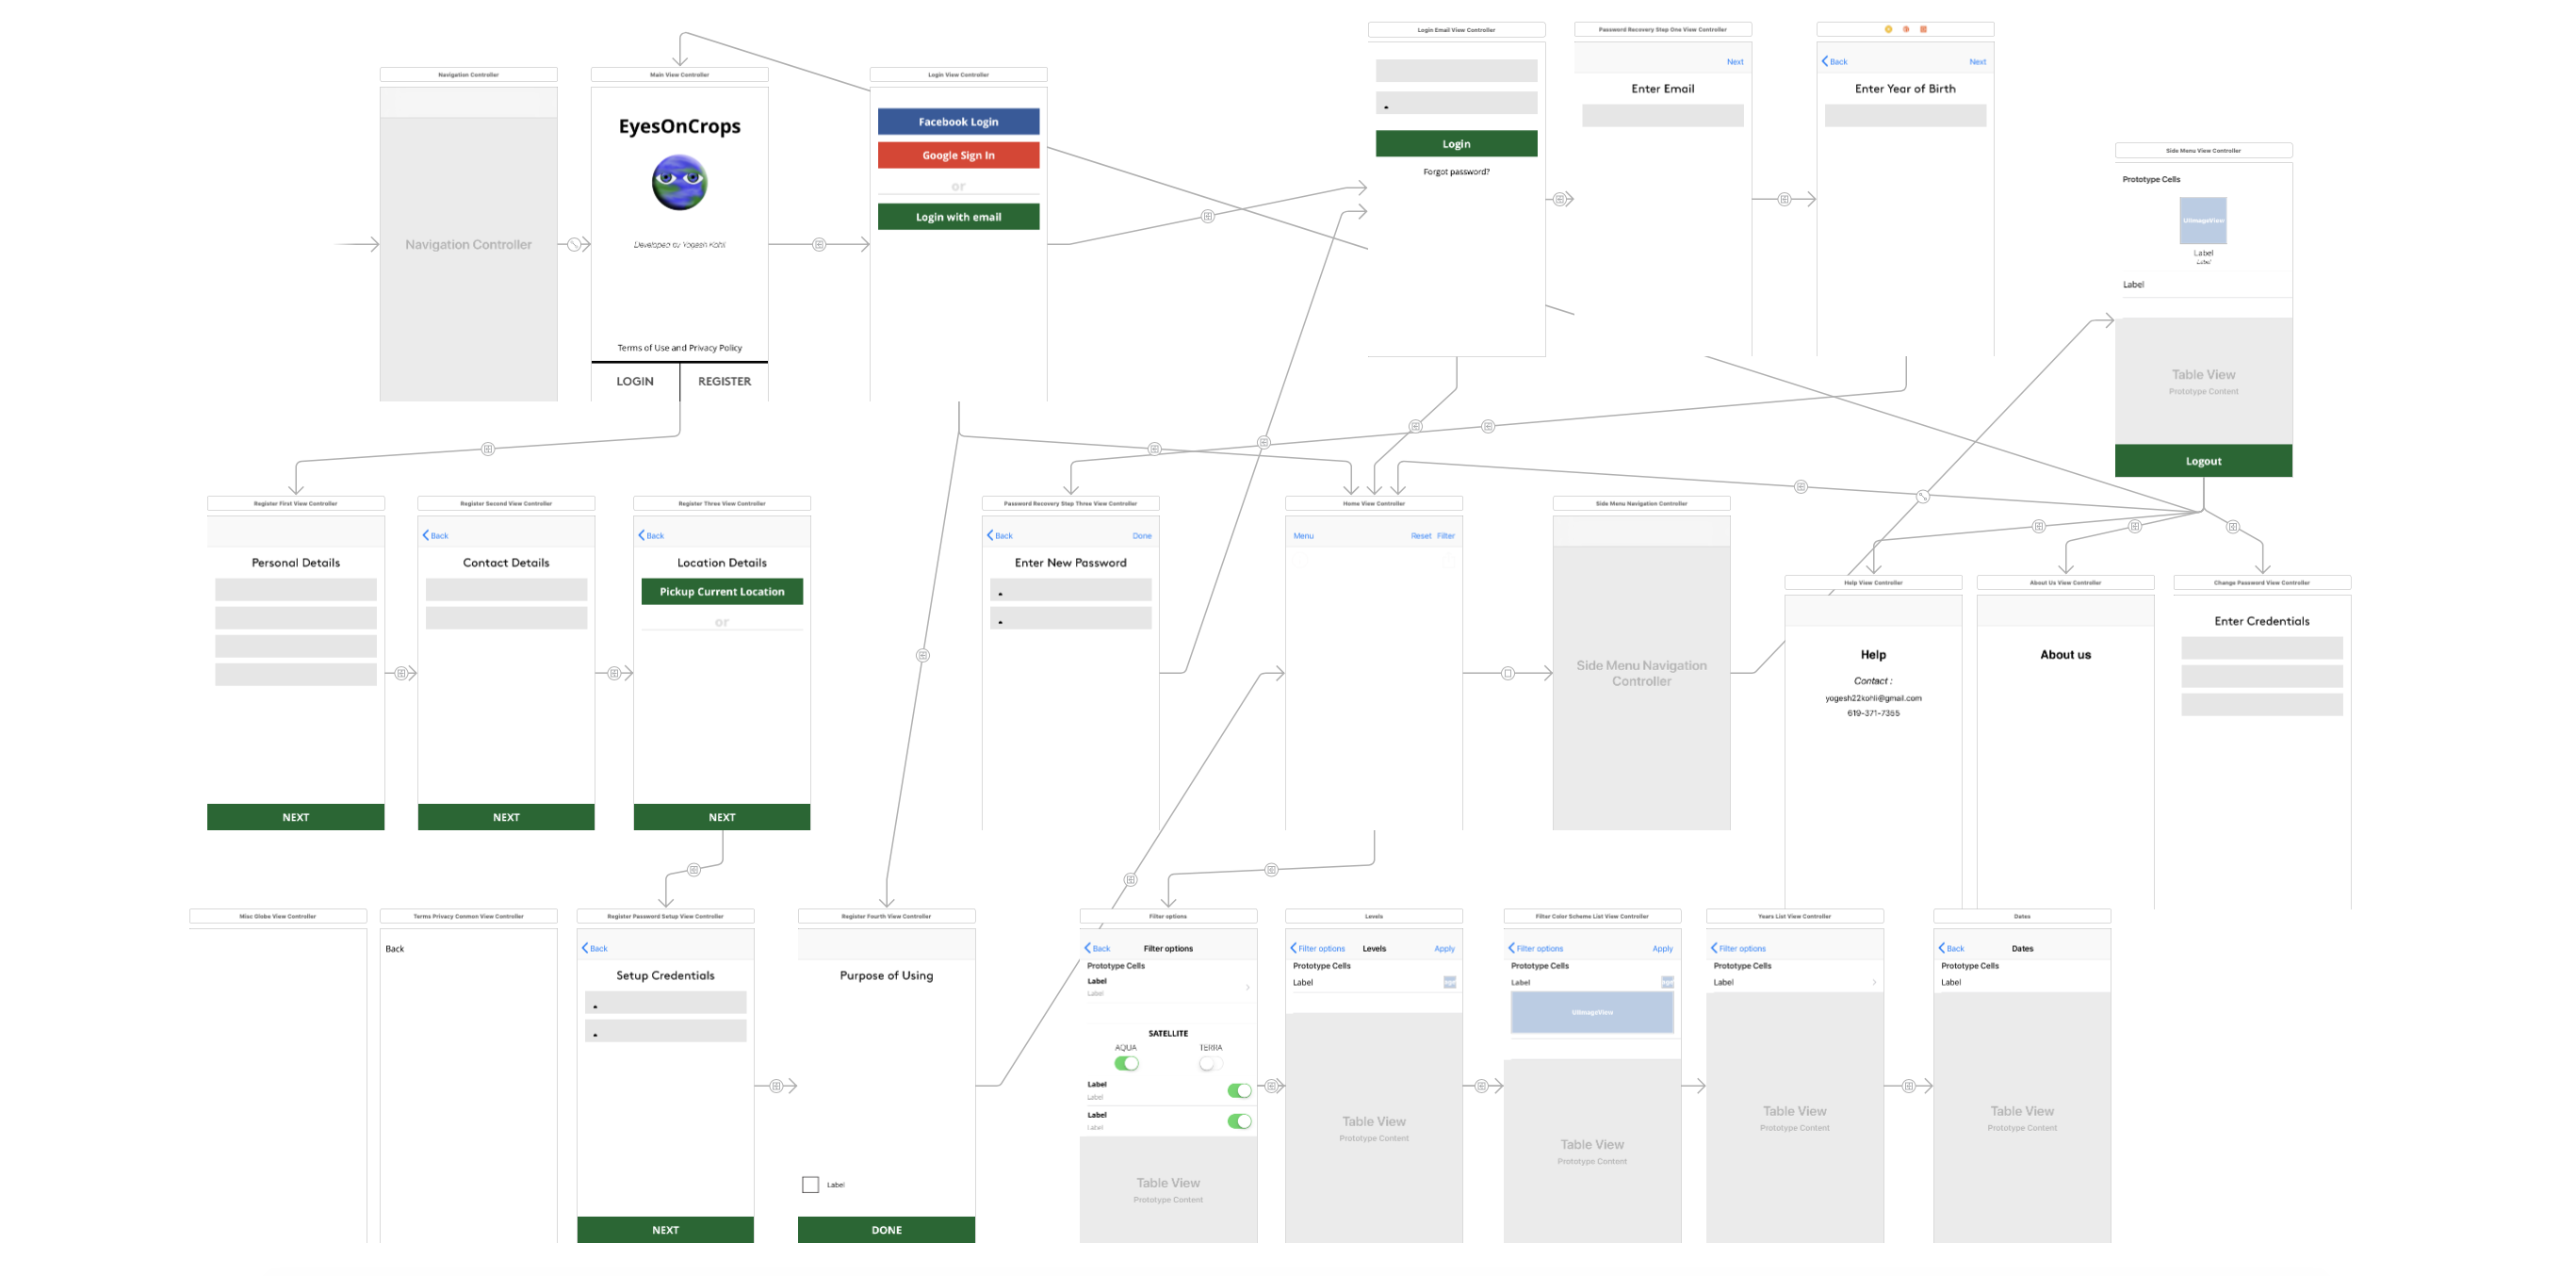
\includegraphics[width=\linewidth]{figures/ch4/storyboard_2.png}
            \caption{\label{fig:wireframe_3} Storyboard of the app}
    \end{figure}
    
\subsection{Mobile App screens and their significance}

\subsubsection{Sign-up via Email}

Sign up process is a one time process which enables you to enter the application out of the blue. It likewise gives us the chance to include the client in our database for future logins and additionally the record.

Sign up via email process consists of 5 screens which are listed below:-

\newpage

\begin{itemize}

    \item Personal details
    
    \begin{figure}[H]
            \centering
            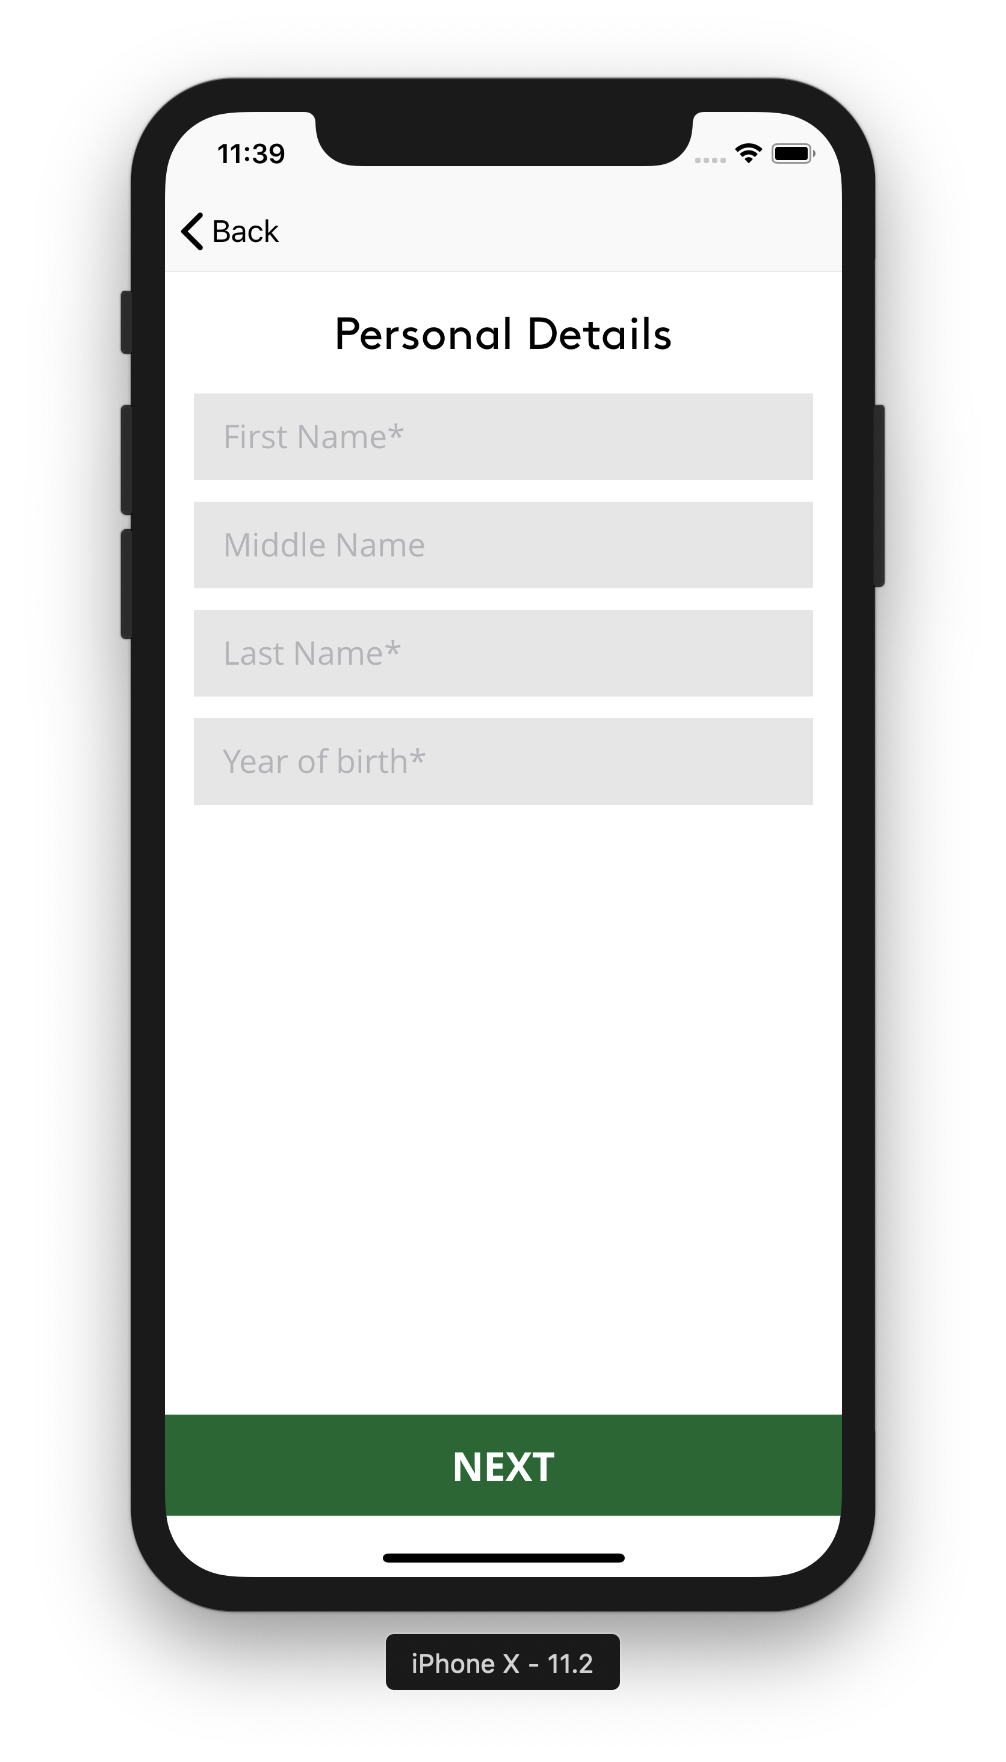
\includegraphics[width=0.4\linewidth]{figures/ch2/register_personal.png}
            \caption{\label{fig:wireframe_3} Register Part-I Personal detail screen}
    \end{figure}
    
    Here in the figure 4.2, mandatory fields are First name, Last name and year of birth where as we have kept middle name as an optional because not everyone has one. \\
    
    UIPickerView is used for selection of year of birth, According to Apple's documentation, UIPickerView is a view that uses a spinning-wheel or slot-machine metaphor to show one or more sets of values.
    
    Figure 4.3 shows the image of the pickerview designed in the app.
    
    \begin{figure}[H]
            \centering
            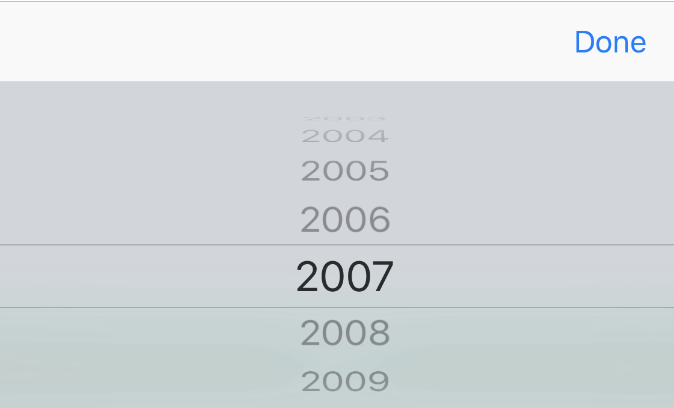
\includegraphics[width=0.4\linewidth]{figures/ch4/pickerview.png}
            \caption{\label{fig:wireframe_3} UIPickerView for year selection}
    \end{figure}
    
    \newpage
    
    \item Contact details
    
    \begin{figure}[H]
            \centering
            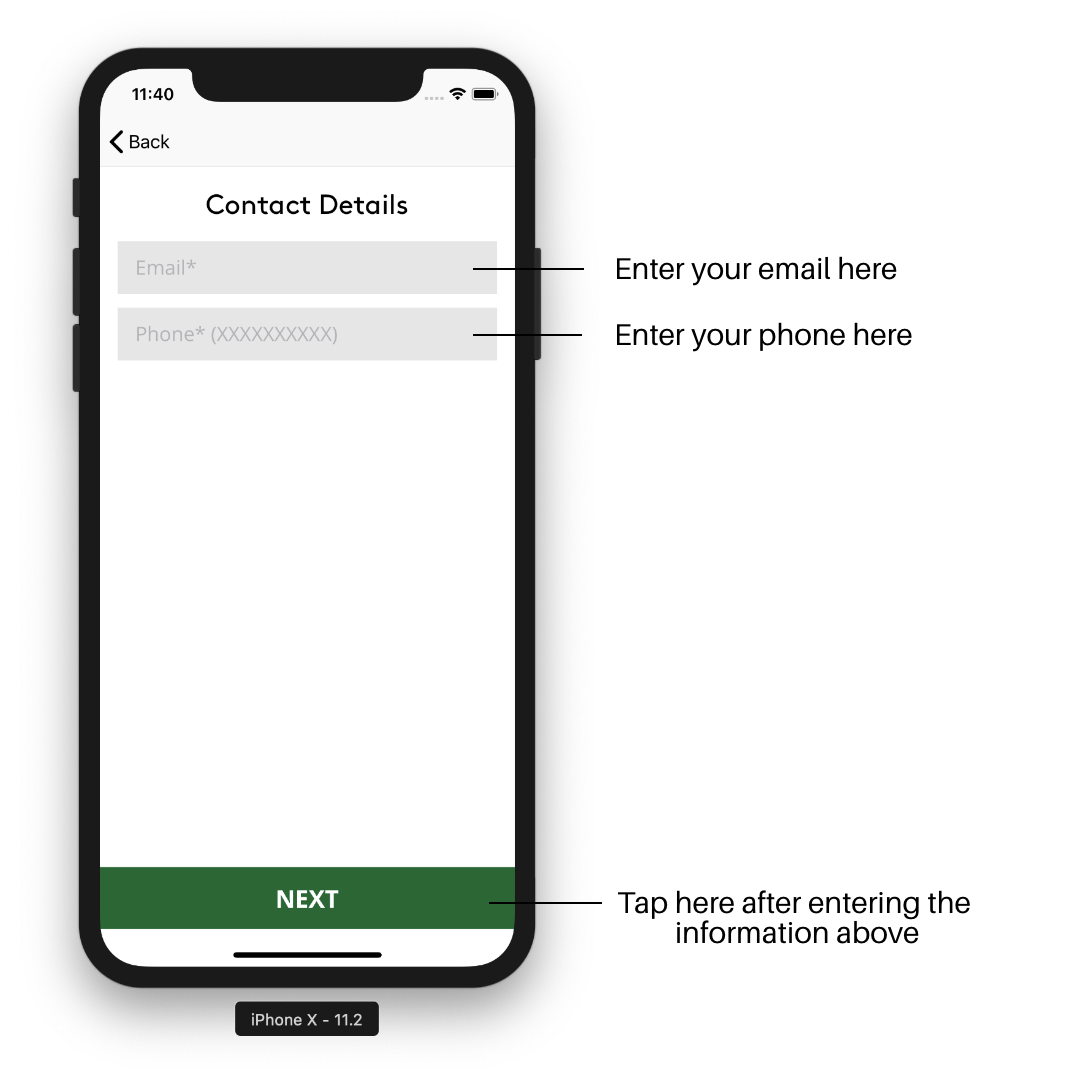
\includegraphics[width=0.5\linewidth]{figures/ch2/register_contact.png}
            \caption{\label{fig:wireframe_3} Register Part-II Contact detail screen}
    \end{figure}
    
    Figure 4.3 represents contact detail screen in which both the fields i.e Email and Phone are mandatory for record purpose and to avoid fake entries. User with unique email and phone can register only once. It's a good point to note that both the fields have been verified syntactically here.
    
    \newpage
  
    \item Location details
    
    \begin{figure}[H]
            \centering
            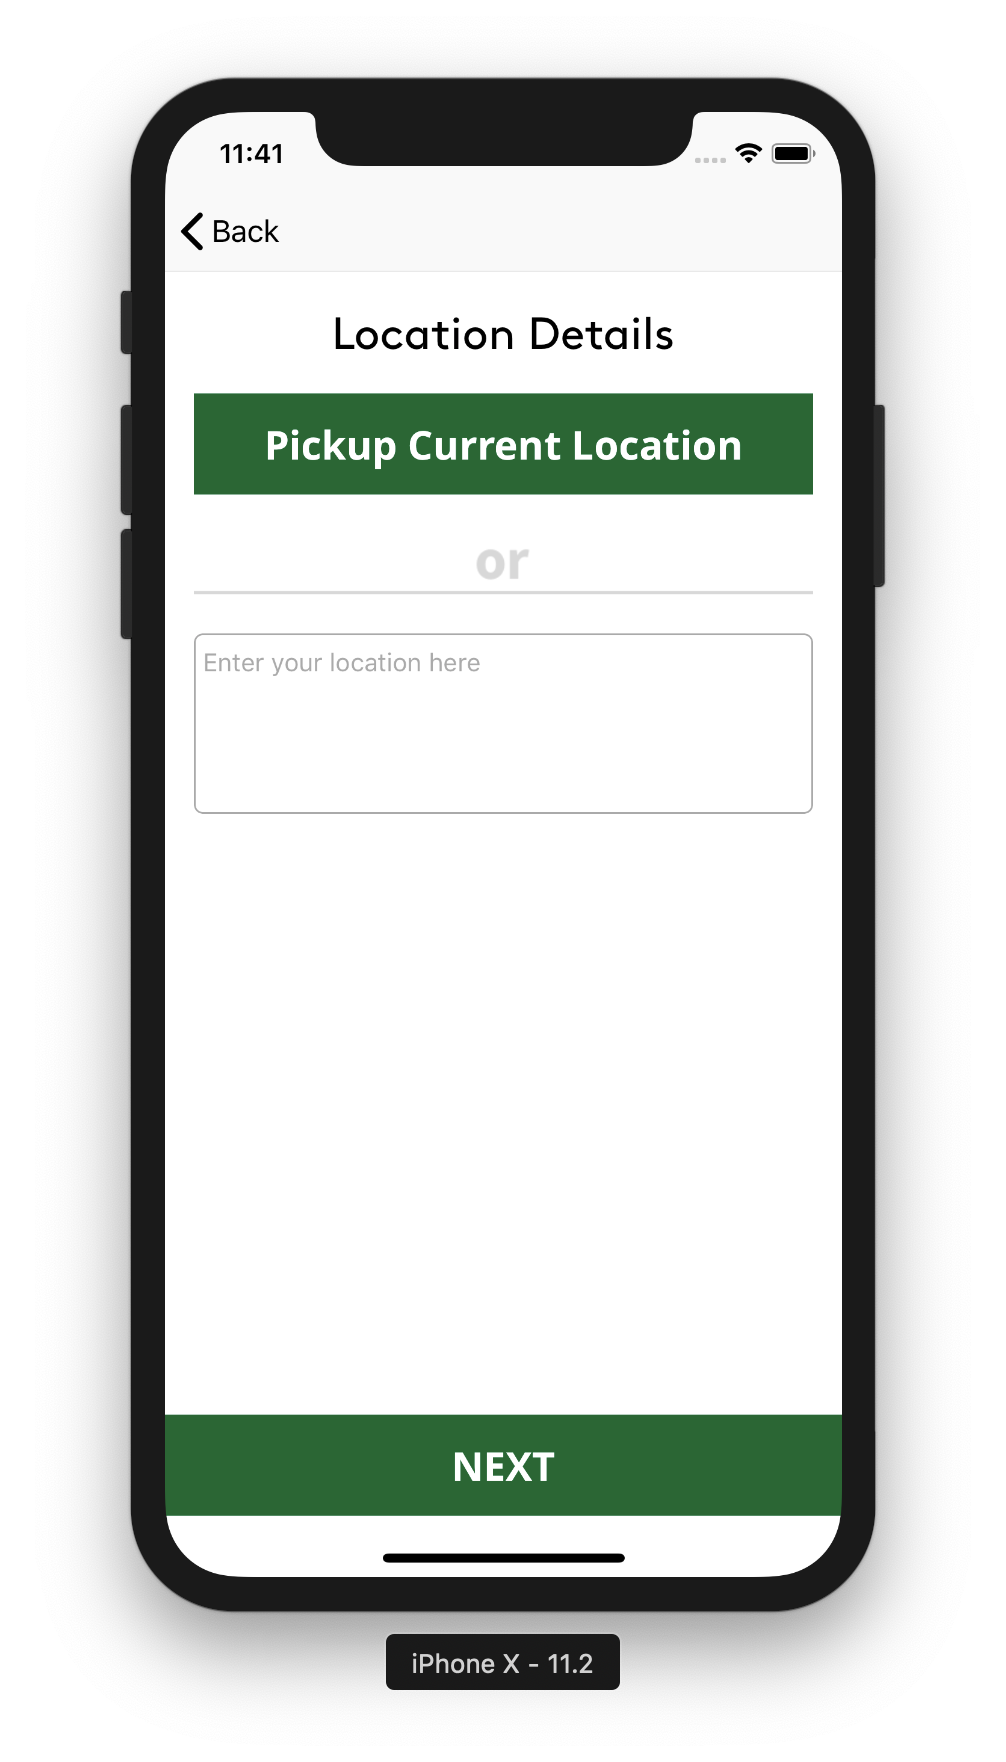
\includegraphics[width=0.5\linewidth]{figures/ch2/register_location.png}
            \caption{\label{fig:wireframe_3} Register Part-III Location detail screen}
    \end{figure}
    
    This screen makes use of Apple's Core Location framework which allows developers to obtain current geographic location of device.
    
    In this screen, user has two possible choices for entering his location, he can enter the area physically or can simply tap on pickup current area which will eventually get the present location and display it in text area showed. Despite everything he can still alter the area if he wants to.
    
    \newpage
    
    \item Setup Credentials
    
    \begin{figure}[H]
            \centering
            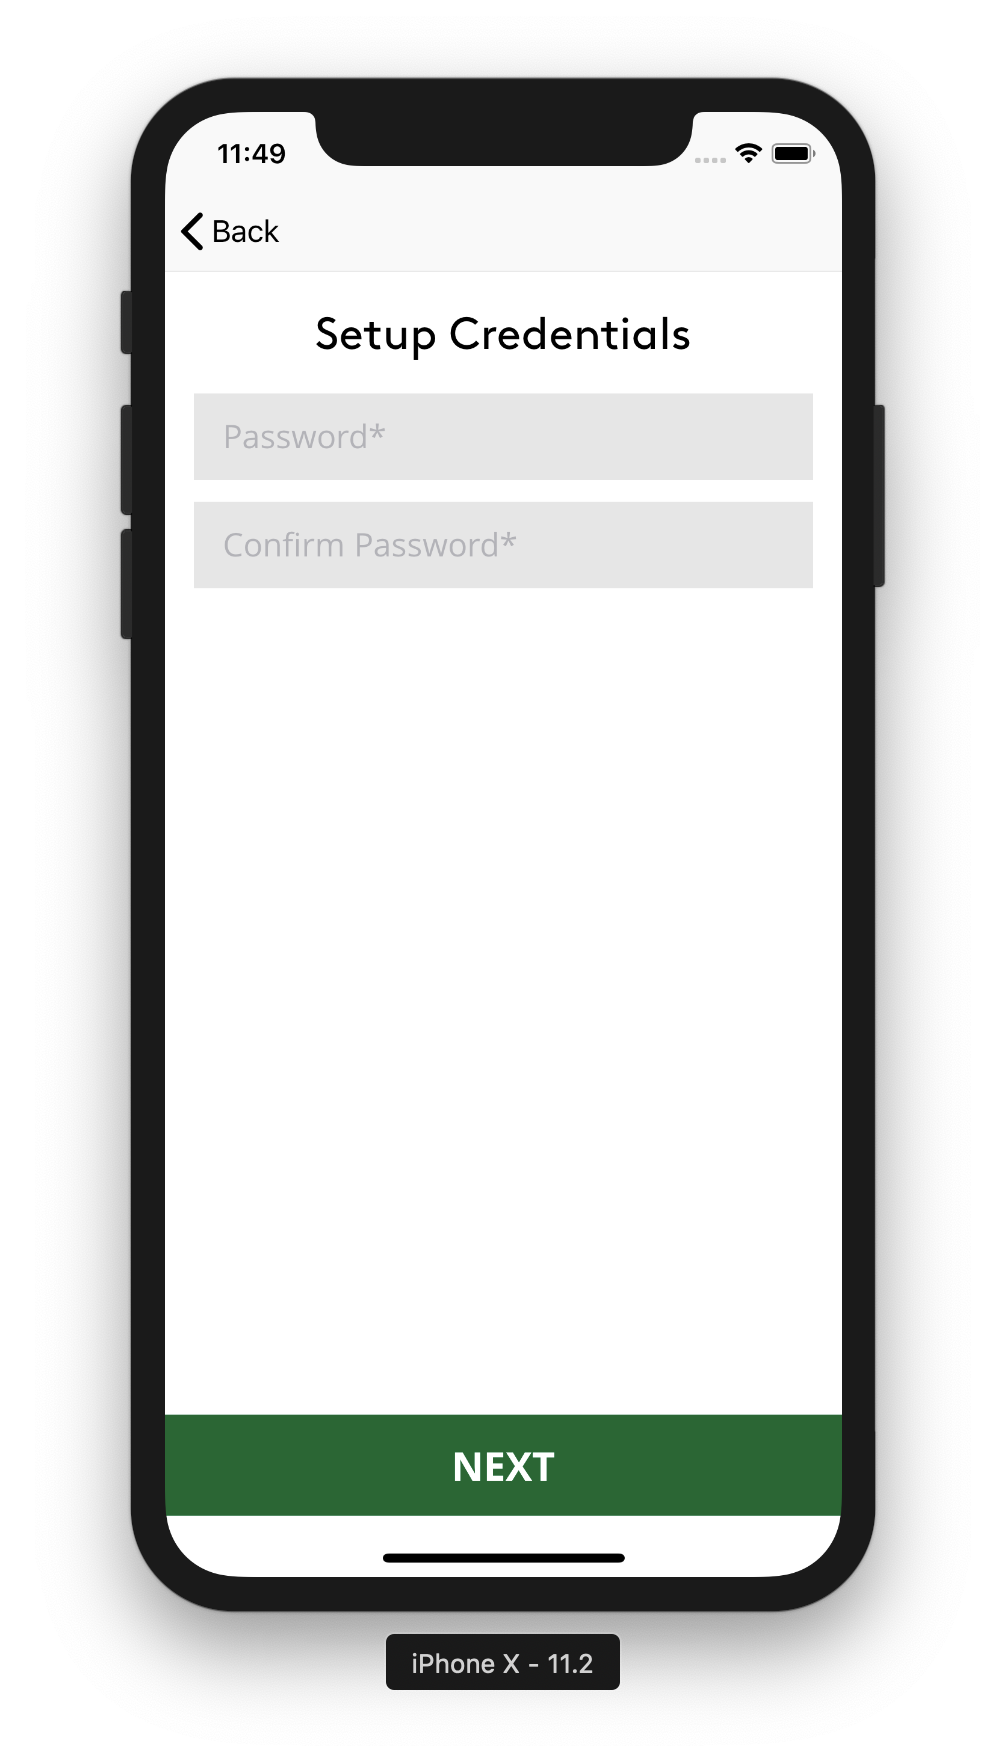
\includegraphics[width=0.5\linewidth]{figures/ch2/credentials_setup.png}
            \caption{\label{fig:wireframe_3} Register Part-IV Credentials setup screen}
    \end{figure}
    
    As you can see in figure 4.6, it allows you to setup password for your secure log in. Point to note here is that minimum length of password has been set 6 digits.
    
    
    \newpage
    
    \item Purpose of using the app
    
     \begin{figure}[H]
            \centering
            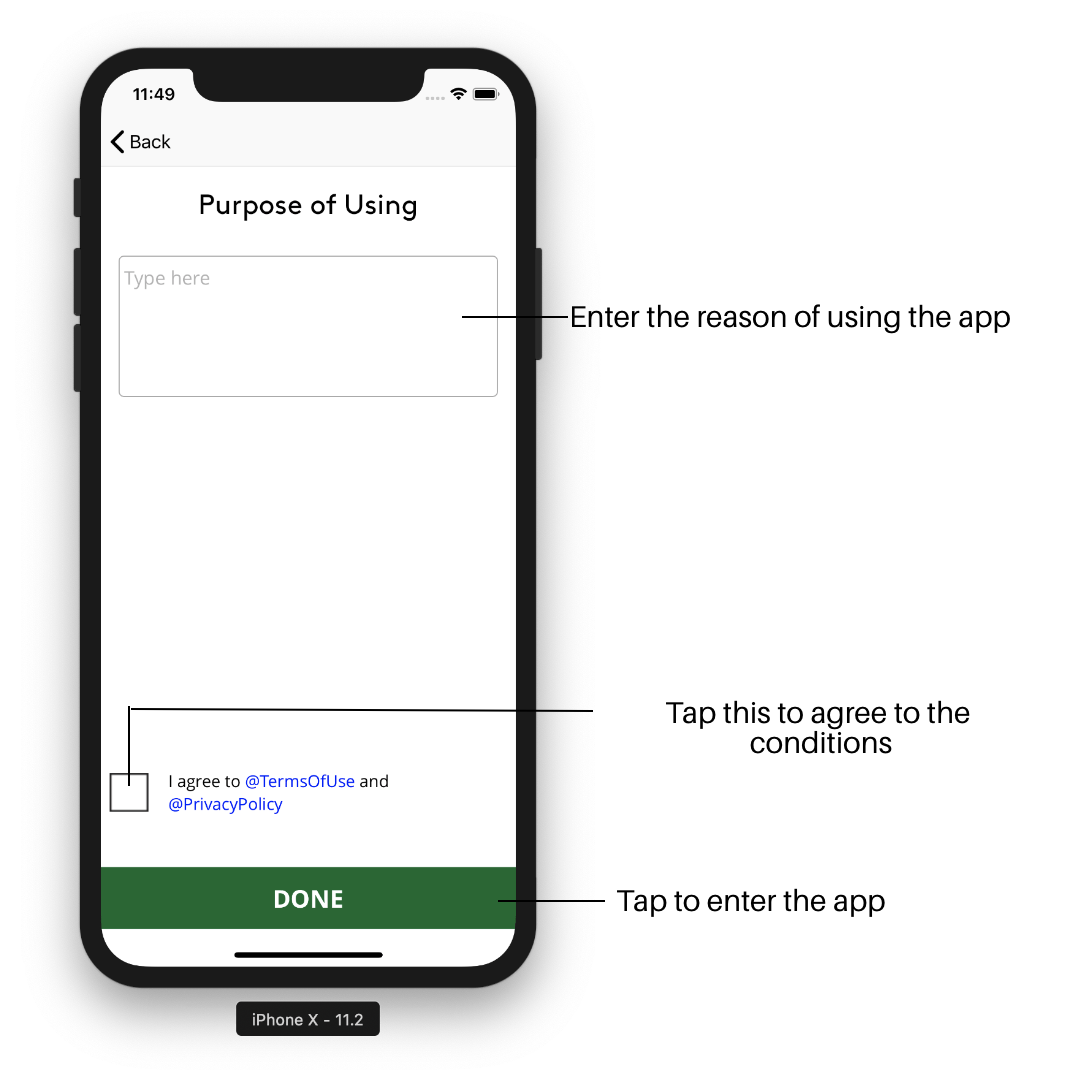
\includegraphics[width=0.5\linewidth]{figures/ch2/purpose_app.png}
            \caption{\label{fig:wireframe_3} Register Part-V Purpose of using the app screen}
    \end{figure}
    
    This screen is really important for us to know what and why people wants to use this app. Moreover, it has additional check mark for privacy policy and terms of use to which every user must agree before going further. It also protects us from some bot attack.
    
    \newpage
 
\end{itemize}


\subsubsection{Login process}

User can log in in the app via certain ways:-

\begin{itemize}
    \item Social Login
    
    \begin{itemize}
        \item Facebook Login
        \item Google Signin
    \end{itemize}
    
    \item Login via email
    
\end{itemize}

\subsubsection{Home screen}
\subsubsection{Sliding Menu}
\subsubsection{Filter process and its sub-screens}

\section{API usage}
\section{Softwares used in making of the app}

Visualization Apps like Argovis have served two purposes. The first purpose is to serve the community; the second is to expand the community. Global data sets in the oceanographic and earth science disciplines could potentially benefit from such apps, with minimal cost to their endeavors. The architecture of Argovis is designed for high traffic demands at low computation by placing visualization loads on the client side. The server side acts as a database and web server only; this allows a relatively high traffic web app be hosted and maintained at a low cost. Moreover, the software used is open source. 

Governmental agencies NOAA and NASA are required to release their data. The amount of data gathered and released is now on the petabyte scale. Without accessibility, this amounts to little more than an archive, accessible only to domain experts. This thesis proposes that agencies and groups design their data interfaces with a user interface in mind. Argovis is designed around the following data acquisition procedure: 
\begin{enumerate}
  \item browse datasets. 
  \item assess its relevance to their needs.
  \item visualize/select their region of interest.
  \item download data in a format they can use.
\end{enumerate}
An additional consideration would be to include a discussion forum to the web app, similar to \url{www.kaggle.com} \cite{kaggle} competitions, where each dataset has its discussion forum, where users post their code, figures and results in \gls{Jupyter} notebooks. Forums allow outside users to contribute to the project. As the institutions themselves may be limited in manpower and funding, they may rely on forums for additional code, tutorials or discussion. For example, Argovis has an API in Python, but users proficient in other scientific languages can write APIs in other languages, such as R, Matlab, and Julia. A forum section of the site works as a source of feedback for the development team. Questions, requests, complaints can be posted and be resolved/answered by either other users or the developers themselves.

The scientific community can become bogged down in data storage problem. Open, community-driven web applications to big data visualization and analysis can help users float on this sea of data.